\section{Silicon, germanium and gallium arsenide}\label{sec:3.3}

The highest occupied electron state of silicon sits at the center of the Brillouin zone, and the lowest empty one sits \SI{85}{\percent} of the way to the square face of the zone, at a crystal momentum of \SI{1.94}{keV}. A photon with the \SI{1.17}{eV} needed to cross the gap carries a momentum a thousand times smaller and cannot connect the two states by itself. A dark-matter particle that scatters with a momentum transfer of a few keV can. Which momentum transfers reach which excitation energies is the target's half of the kinematic question of \cref{sec:1.3}, and the answer lies in the bands just below and just above the gap. \Cref{tab:3-materials} collects the band edges, effective masses and spin--orbit splittings of silicon, germanium and GaAs, the book's running materials.

\subsection{Band edges and valleys}

At the temperatures at which detectors run, the four lowest bands of silicon are full and all higher bands are empty (\cref{sec:3.2}). The full bands are the \emph{valence bands} and the empty ones the \emph{conduction bands}. We label them with the subscripts $v$ and $c$, as in $\varepsilon_{v\vect{k}}$ and $\varepsilon_{c\vect{k}}$, and the two letters never appear on their own. The highest valence energy is the \emph{valence-band maximum} (VBM), and the lowest conduction energy the \emph{conduction-band minimum} (CBM). The band gap is the distance between the two,
\begin{equation}
  \Eg = \min_{c,\vect{k}}\varepsilon_{c\vect{k}} - \max_{v,\vect{k}}\varepsilon_{v\vect{k}} ,
  \label{eq:3.3-Eg}
\end{equation}
wherever in the zone the two extremes occur. When they occur at different crystal momenta the gap is \emph{indirect}. A transition at fixed crystal momentum is called \emph{vertical}, after its appearance in a band diagram, and the smallest vertical transition energy is the \emph{minimum direct gap},
\begin{equation}
  E_{\mathrm{dir}} = \min_{v,c,\vect{k}}\left(\varepsilon_{c\vect{k}} - \varepsilon_{v\vect{k}}\right) \ge \Eg .
  \label{eq:3.3-Edir}
\end{equation}
In a direct-gap crystal the two are equal.

\Cref{fig:3-si-bands}(a) shows the bands of silicon along the lines of \cref{sec:3.1}. The VBM lies at $\mathrm{\Gamma}$ and is threefold degenerate, sixfold with spin. These are the bonding states of the $sp^3$ picture of \cref{sec:3.2} with pure $p$ character: the three states transform like $x$, $y$ and $z$ under the rotations of the crystal, and an $s$ orbital, unchanged by every rotation, cannot enter them. The CBM lies on the line from $\mathrm{\Gamma}$ to $\mathrm{X}$, at the crystal momentum
\begin{equation}
  \vect{k}_{\mathrm{c}} = 0.85\,\frac{2\pi}{a}\,(1, 0, 0)
  \label{eq:3.3-kc}
\end{equation}
and at the five equivalent points along $\pm x$, $\pm y$ and $\pm z$; the position was measured by electron--nuclear double resonance on donor electrons, which occupy these states~\cite{feher1959electron}. The six minima are the \emph{valleys} of the conduction band. An electron excited across the gap relaxes into one of them, and near its bottom it behaves like a free particle with an anisotropic mass, which we derive below. The gap is $\Eg = \SI{1.17}{eV}$ at low temperature, $\SI{1.1692}{eV}$ in the extrapolation to zero temperature~\cite[Eq.~(11)]{ramanathan2020ionization}, and \SI{1.12}{eV} at \SI{300}{K}~\cite[Table~I]{lucero2012improved}. It shrinks on warming because the lattice expands and the electron--phonon interaction renormalizes the band energies (\cref{sec:13.7}). The vertical transitions of silicon cost much more. The smallest, $E_{\mathrm{dir}} = \SI{3.4}{eV}$, joins the valence and conduction states at $\mathrm{\Gamma}$~\cite[Table~II]{rideau2006strained}, and vertical transitions near $\mathrm{L}$ start only slightly higher, at \SI{3.45}{eV}~\cite[Table~VI]{rideau2006strained}. Silicon is thus indirect by a wide margin, $E_{\mathrm{dir}} \approx 3\Eg$.

\begin{figure}[tbp]
  \centering
  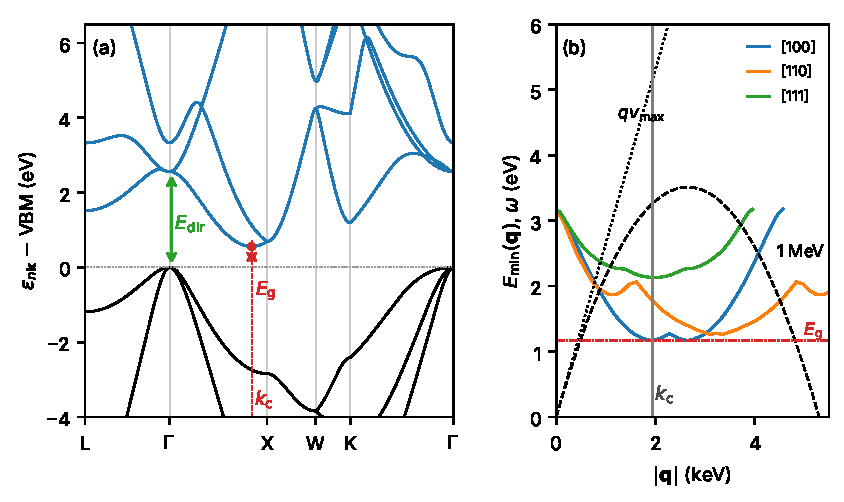
\includegraphics[width=\linewidth]{figures/ch03/fig3_6.pdf}
  \caption{Silicon. (a)~Band structure along $\mathrm{L}$--$\mathrm{\Gamma}$--$\mathrm{X}$--$\mathrm{W}$--$\mathrm{K}$--$\mathrm{\Gamma}$ (points of \cref{sec:3.1}), valence bands black and conduction bands blue, energies from the valence-band maximum. The bands are the Kohn--Sham bands of the plane-wave calculation of \cref{app:E.1} at the measured lattice constant: generalized-gradient functional of Perdew, Burke and Ernzerhof (PBE), SG15 norm-conserving pseudopotential, cutoff \SI{60}{Ry}, $12^3$ grid for the density, $a = \SI{5.431}{\angstrom}$, no spin--orbit coupling~\cite{giannozzi2017advanced,hamann2013optimized,schlipf2015optimization}. They put the conduction-band minimum at $k_{\mathrm{c}} = 0.843\,(2\pi/a)$ (measured $0.85$) and the indirect gap $\Eg$ at \SI{0.557}{eV} (measured \SI{1.17}{eV}), the gap problem of density-functional theory. The vertical gap at $\mathrm{\Gamma}$, marked $E_{\mathrm{dir}}$, is \SI{2.56}{eV} (measured \SI{3.4}{eV}) and is the smallest vertical gap in the zone; the one at $\mathrm{L}$ is \SI{2.70}{eV} (measured \SI{3.45}{eV}). (b)~Minimum pair energy $E_{\mathrm{min}}(\vect{q})$, \cref{eq:3.3-Emin}, for $\vect{q}$ along [100], [110] and [111], from the same calculation on a grid of $48^3$ crystal momenta, with the conduction bands shifted rigidly up by \SI{0.61}{eV} (a scissor, \cref{sec:3.4}) so that the indirect gap equals the measured \SI{1.17}{eV} (dash-dotted line); at $\vect{q} = 0$ the shifted bands give $E_{\mathrm{min}} = \SI{3.17}{eV}$. Dashed: the largest energy that dark matter of \SI{1}{MeV} can deposit, $qv_{\mathrm{max}} - q^2/2\mchi$; dotted: the bound $qv_{\mathrm{max}}$ for any mass, with $v_{\mathrm{max}} = 2.650\times10^{-3}$. The vertical line marks $|\vect{k}_{\mathrm{c}}| = \SI{1.94}{keV}$. Along [100], $E_{\mathrm{min}}$ returns to its value at $\vect{q} = 0$ at $|\vect{G}_{200}| = \SI{4.57}{keV}$.}
  \label{fig:3-si-bands}
\end{figure}

Germanium has the same diamond structure, with $a = \SI{5.658}{\angstrom}$ at room temperature~\cite[Sect.~II\,A]{rideau2006strained}, and the same threefold VBM at $\mathrm{\Gamma}$. Its CBM, however, lies at $\mathrm{L}$, the center of a hexagonal face of the zone (\cref{fig:3-ge-gaas}(a)). The eight $\mathrm{L}$ points come in pairs that differ by a vector $\vect{G}_{111}$ and are the same crystal momentum, so germanium has four valleys, each made of two half-ellipsoids on opposite faces of the zone. The gap is \SI{0.744}{eV} at low temperature~\cite[Table~VI]{rideau2006strained} and \SI{0.66}{eV} at \SI{300}{K}~\cite[Table~I]{lucero2012improved}. The conduction state at $\mathrm{\Gamma}$ is only \SI{0.15}{eV} higher, $E_{\mathrm{dir}} = \SI{0.89}{eV}$~\cite[Table~II]{rideau2006strained}: germanium is indirect by a narrow margin, and a calculation can easily get the order of the two states wrong.

GaAs has the zincblende structure, with $a = \SI{5.653}{\angstrom}$ at room temperature~\cite{vurgaftman2001band}, and both band edges at $\mathrm{\Gamma}$ (\cref{fig:3-ge-gaas}(b)). Its gap is direct, \SI{1.52}{eV} at low temperature and \SI{1.42}{eV} at \SI{300}{K}~\cite[Table~I]{lucero2012improved}, and the conduction band has a single, isotropic valley. Valleys at $\mathrm{L}$ and $\mathrm{X}$ follow at 1.815 and \SI{1.981}{eV}, 0.30 and \SI{0.46}{eV} above the minimum~\cite{vurgaftman2001band}. Gallium and arsenic flank germanium in the periodic table, yet the gap of GaAs is twice that of germanium. The difference comes from the partly ionic bond of \cref{sec:3.2}: the two hybrids of a bond have different energies, and this difference adds to their covalent splitting.

\begin{figure}[tbp]
  \centering
  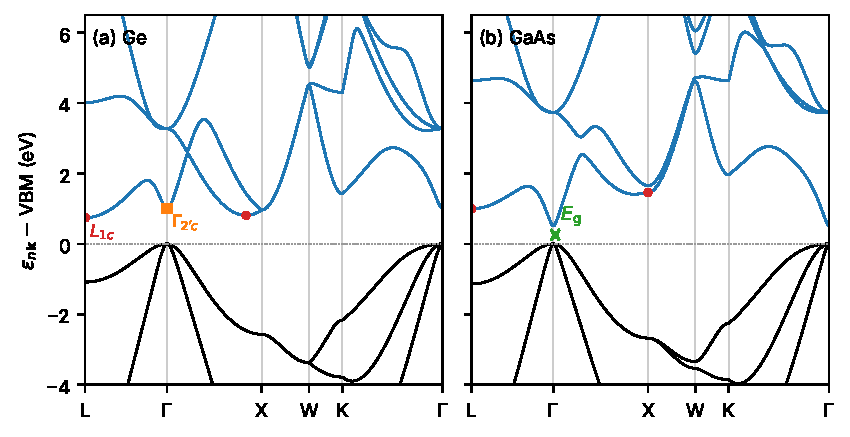
\includegraphics[width=\linewidth]{figures/ch03/fig3_7.pdf}
  \caption{Band structures of (a)~germanium and (b)~GaAs along the path of \cref{fig:3-si-bands}(a). Energies from the valence-band maximum; red dots mark the lowest conduction states away from $\mathrm{\Gamma}$. (a)~Local empirical pseudopotential of Cohen and Bergstresser~\cite{cohen1966band} at $a = \SI{5.66}{\angstrom}$, the lattice constant of their fit, without spin--orbit coupling, with the conduction bands shifted down by \SI{0.21}{eV} so that the $\mathrm{L}$ minimum sits at the measured \SI{0.744}{eV}. The crystal is indirect, with the $s$-like state $\mathrm{\Gamma}_{2'c}$ (square) at \SI{1.01}{eV} (measured \SI{0.89}{eV}) and the $\Delta$ minimum, at $0.83\,(2\pi/a)$ along $\mathrm{\Gamma}$--$\mathrm{X}$, at \SI{0.81}{eV}. Plain PBE with spin--orbit coupling at the measured lattice constant closes the germanium gap, with $\mathrm{\Gamma}_{7c}$ \SI{0.05}{eV} below the valence maximum. (b)~PBE plane-wave calculation of \cref{fig:3-si-bands} (SG15 pseudopotentials with the Ga $3d$ shell in the valence, \SI{60}{Ry}, $12^3$ grid, no spin--orbit coupling) at the room-temperature lattice constant $a = \SI{5.653}{\angstrom}$~\cite{giannozzi2017advanced,hamann2013optimized,schlipf2015optimization}. The gap is direct, as measured, but PBE underestimates it: \SI{0.51}{eV} against the measured \SI{1.52}{eV} at low temperature, with the $\mathrm{L}$ and $\mathrm{X}$ states at 1.00 and \SI{1.46}{eV} (measured 1.815 and \SI{1.981}{eV}).}
  \label{fig:3-ge-gaas}
\end{figure}

The bands in \cref{fig:3-si-bands} and \cref{fig:3-ge-gaas}(b) come from density-functional theory, which yields the potential from the electron density. A second route, which we use for the germanium bands of \cref{fig:3-ge-gaas}(a) and below as a model to test the velocity sum rules, is the empirical pseudopotential. It solves the central equation \cref{eq:3.2-central} with a potential that has nonzero Fourier components $U_{\vect{G}}$ on just the three shortest shells of reciprocal-lattice vectors, and fits these three numbers per element to measured optical transitions~\cite{cohen1966band}. That the fit works at all shows how much of the band structure the lattice fixes and how little of the potential it needs; the price is that the potential is not computed but adjusted, and it says nothing about wavefunctions at large momentum. Its potential is local, which is what makes it a convenient test bed for the sum rules. The band parameters of \cref{tab:3-materials} are measured. A first-principles calculation is checked against exactly these numbers: the measured gaps, the valley positions, the masses from cyclotron resonance, and the electronic dielectric constant of silicon, $\varepsilon_\infty = 11.7$, the square of its long-wavelength refractive index, 3.42~\cite{li1980refractive} (\cref{sec:4.4}). For the gaps the comparison needs one more step, a \emph{quasiparticle correction} that turns the Kohn--Sham eigenvalues into the energies to add or remove an electron (\cref{app:E.3}). The PBE functional of \cref{fig:3-si-bands} is \emph{semilocal}: its exchange--correlation energy at each point depends on the density and its gradient there and nowhere else. It places the CBM of silicon at $k_{\mathrm{c}} = 0.843\,(2\pi/a)$ and its longitudinal mass, $0.95\,m_e$, within \SI{4}{\percent} of experiment, but it puts the gap at \SI{0.56}{eV}, half the measured one.

\begin{table}[tbp]
  \centering
  \caption{Band parameters of silicon, germanium and GaAs. Lattice constant $a$ at room temperature: silicon~\cite[lattice parameter of silicon]{mohr2025codata}, germanium~\cite[Sect.~II\,A]{rideau2006strained}, GaAs~\cite{vurgaftman2001band}. Gaps at low temperature: silicon~\cite[Eq.~(11)]{ramanathan2020ionization}, germanium~\cite[Table~VI]{rideau2006strained}, GaAs~\cite[Table~I]{lucero2012improved}; at \SI{300}{K}~\cite[Table~I]{lucero2012improved}. Minimum direct gaps $E_{\mathrm{dir}}$ and spin--orbit splittings $\Delta_{\mathrm{SO}}$ of silicon and germanium~\cite[Table~II]{rideau2006strained}. Conduction valleys: position and number; masses along ($m^*_\parallel$) and across ($m^*_\perp$) the valley axis, silicon~\cite{hensel1965cyclotron} as listed in Ref.~\cite[Table~VII]{rideau2006strained}, germanium~\cite[Table~VII]{rideau2006strained}. Heavy- and light-hole masses $m_{\mathrm{hh}}$, $m_{\mathrm{lh}}$ along [100] and [111] from \cref{eq:3.3-holes} with the Luttinger parameters $(\gamma^{\mathrm{Lu}}_1, \gamma^{\mathrm{Lu}}_2, \gamma^{\mathrm{Lu}}_3) = (4.285, 0.339, 1.446)$ for silicon and $(13.25, 4.20, 5.56)$ for germanium~\cite[Table~VII]{rideau2006strained}, and $(6.98, 2.06, 2.93)$ for GaAs. All GaAs entries not credited otherwise are from Ref.~\cite{vurgaftman2001band}. Masses in units of $m_e$.}
  \label{tab:3-materials}
  \small
  \begin{tabular}{l ccc}
    \toprule
    & Si & Ge & GaAs \\
    \midrule
    $a$ (\AA) & 5.431 & 5.658 & 5.653 \\
    $\Eg$, low $T$ / \SI{300}{K} (eV) & 1.17 / 1.12 & 0.744 / 0.66 & 1.52 / 1.42 \\
    gap & indirect & indirect & direct \\
    $E_{\mathrm{dir}}$ (eV) & 3.4 & 0.89 & 1.52 \\
    valleys & $0.85\,\mathrm{X}$, 6 & $\mathrm{L}$, 4 & $\mathrm{\Gamma}$, 1 \\
    $m^*_\parallel$ / $m^*_\perp$ & 0.916 / 0.191 & 1.59 / 0.0815 & 0.067 (isotropic) \\
    $\Delta_{\mathrm{SO}}$ (eV) & 0.044 & 0.296 & 0.341 \\
    $m_{\mathrm{hh}}$ [100] / [111] & 0.277 / 0.718 & 0.206 / 0.469 & 0.350 / 0.893 \\
    $m_{\mathrm{lh}}$ [100] / [111] & 0.201 / 0.139 & 0.046 / 0.041 & 0.090 / 0.078 \\
    \bottomrule
  \end{tabular}
\end{table}

A gap of an electronvolt is enormous compared with the temperature of a detector, and the number of electrons excited across it by heat alone is a useful check of what ``empty'' means. Far from the chemical potential $\mu_{\mathrm{ch}}$ the occupation \cref{eq:3.2-fnk} of a conduction state is the Boltzmann factor $\ee^{-(\varepsilon_{c\vect{k}} - \mu_{\mathrm{ch}})/T}$. For a parabolic band of mass $m$ its sum over crystal momenta, $\int\dd^3k\,(2\pi)^{-3}\ee^{-k^2/2mT} = (mT/2\pi)^{3/2}$, times 2 for spin, gives the electron density $2(m_{\mathrm{dc}}T/2\pi)^{3/2}$ times the Boltzmann factor of the CBM. The empty valence states, the holes, give the same expression with the valence mass and the factor $\ee^{-(\mu_{\mathrm{ch}} - \varepsilon_{\mathrm{VBM}})/T}$. In a pure crystal the two densities are equal, the chemical potential drops out of their product, and the \emph{intrinsic carrier density} is~\cite[Chap.~28]{ashcroft1976solid}
\begin{equation}
  \nd_{\mathrm{i}} = 2\left(\frac{T}{2\pi}\right)^{3/2}(m_{\mathrm{dc}}m_{\mathrm{dv}})^{3/4}\,\ee^{-\Eg/2T} .
  \label{eq:3.3-ni}
\end{equation}
Here $m_{\mathrm{dc}}$ and $m_{\mathrm{dv}}$ are the density-of-states masses of the conduction and valence bands: for silicon $m_{\mathrm{dc}} = 6^{2/3}(m^*_\parallel m^{*2}_\perp)^{1/3} = 1.06\,m_e$, which counts the six valleys, and $m_{\mathrm{dv}} = (m_{\mathrm{hh}}^{3/2} + m_{\mathrm{lh}}^{3/2})^{2/3} = 0.50\,m_e$, which adds the heavy and light holes with their spherically averaged masses $m_e/(\gamma^{\mathrm{Lu}}_1 \mp 2\bar\gamma^{\mathrm{Lu}})$, $\bar\gamma^{\mathrm{Lu}} = (2\gamma^{\mathrm{Lu}}_2 + 3\gamma^{\mathrm{Lu}}_3)/5$, from the Luttinger parameters of \cref{eq:3.3-holes} below. At \SI{300}{K}, with $\Eg = \SI{1.12}{eV}$, \cref{eq:3.3-ni} yields $\nd_{\mathrm{i}} \approx \SI{6e9}{cm^{-3}}$ for parabolic bands. With the low-temperature gap it falls to $10^{-20}\,\si{cm^{-3}}$ at \SI{77}{K} and to $10^{-720}\,\si{cm^{-3}}$ at \SI{4}{K}. A kilogram of silicon has a volume of \SI{429}{cm^3}, so a cold crystal holds no thermally excited carriers at all, and the dark counts of a charge detector (\cref{sec:1.5}) come from other sources.

\subsection{Effective masses from \texorpdfstring{$\vect{k}\cdot\vect{p}$}{k.p} theory}

Near the bottom of a valley the band is a quadratic function of the distance $\delta\vect{k} = \vect{k} - \vect{k}_0$ from the minimum $\vect{k}_0$. Its curvature decides how an electron there moves, and how many states lie within an energy $\omega$ of the edge. The curvature follows from the states at $\vect{k}_0$ alone. With \cref{eq:3.2-Hk}, the Bloch Hamiltonian a little away from $\vect{k}_0$ is
\begin{equation*}
  H_{\vect{k}_0+\delta\vect{k}} = \frac{(\op{\vect{p}} + \vect{k}_0 + \delta\vect{k})^2}{2m_e} + U(\vect{r})
  = H_{\vect{k}_0} + \delta\vect{k}\cdot\frac{\op{\vect{p}} + \vect{k}_0}{m_e} + \frac{|\delta\vect{k}|^2}{2m_e} .
\end{equation*}
The operator multiplying $\delta\vect{k}$ is $\nabla_{\vect{k}}H_{\vect{k}}$ at $\vect{k}_0$, whose matrix elements between the periodic parts are the velocity matrix elements $\vect{v}_{mn}(\vect{k}_0)$ of \cref{eq:3.2-dHk}. Treating the two $\delta\vect{k}$-dependent terms as a perturbation of $H_{\vect{k}_0}$, whose eigenstates are the $u_{m\vect{k}_0}$, and going to second order in $|\delta\vect{k}|$ for a nondegenerate band $n$,
\begin{equation}
  \varepsilon_{n,\vect{k}_0+\delta\vect{k}} = \varepsilon_{n\vect{k}_0} + \delta\vect{k}\cdot\vect{v}_{nn} + \frac{|\delta\vect{k}|^2}{2m_e}
  + \sum_{m\neq n}\frac{|\delta\vect{k}\cdot\vect{v}_{mn}|^2}{\varepsilon_{n\vect{k}_0} - \varepsilon_{m\vect{k}_0}} + O(|\delta\vect{k}|^3) ,
  \label{eq:3.3-kp}
\end{equation}
with all velocities at $\vect{k}_0$. The linear term is the group velocity \cref{eq:3.2-vg}, which vanishes at an extremum. Writing $|\delta\vect{k}\cdot\vect{v}_{mn}|^2 = \sum_{\alpha\beta}\delta k_\alpha\,\delta k_\beta\,v^\alpha_{nm}v^\beta_{mn}$, with $v^\alpha_{nm} = (v^\alpha_{mn})^*$, and comparing with $\varepsilon_{n\vect{k}_0} + \frac12\sum_{\alpha\beta}\delta k_\alpha(m^{*-1})_{\alpha\beta}\delta k_\beta$:
\begin{keyresult}[Effective mass from $\vect{k}\cdot\vect{p}$ theory]
At a nondegenerate extremum $\vect{k}_0$ of band $n$, the inverse effective-mass tensor is
\begin{equation}
  (m^{*-1})_{\alpha\beta} \equiv \frac{\partial^2\varepsilon_{n\vect{k}}}{\partial k_\alpha\,\partial k_\beta}
  = \frac{\delta_{\alpha\beta}}{m_e} + 2\sum_{m\neq n}\frac{\Real\bigl[v^\alpha_{nm}(\vect{k}_0)\,v^\beta_{mn}(\vect{k}_0)\bigr]}{\varepsilon_{n\vect{k}_0} - \varepsilon_{m\vect{k}_0}} ,
  \label{eq:3.3-mass}
\end{equation}
and near the extremum $\varepsilon_{n,\vect{k}_0+\delta\vect{k}} = \varepsilon_{n\vect{k}_0} + \frac12\,\delta\vect{k}\cdot m^{*-1}\delta\vect{k}$.
\end{keyresult}
The same result follows from differentiating the group velocity \cref{eq:3.2-vg} once more and using \cref{eq:3.2-dudk}, which is how $\vect{k}\cdot\vect{p}$ theory is usually presented~\cite[Chap.~2]{yu2010fundamentals}. For a nonlocal potential the term $\delta_{\alpha\beta}/m_e$ becomes the expectation value of $\partial^2H_{\vect{k}}/\partial k_\alpha\partial k_\beta$, while the sum keeps its form with the velocities of \cref{eq:3.2-dHk}.

\Cref{eq:3.3-mass} reads like level repulsion. Every other band $m$ pushes band $n$ away from itself as $\vect{k}$ moves, and pushes harder the closer it lies and the larger the velocity matrix element between the two. Bands below a conduction minimum push it up on both sides and make it light; bands above a valence maximum push it down and make the hole light. A small gap therefore means a light mass, provided the velocity matrix element across it is sizable.

Silicon provides a check. The sum rule is exact only for a local potential, so we test it in the empirical pseudopotential of Cohen and Bergstresser described above. The model has form factors of $-0.21$, $+0.04$ and $+0.08$~Ry on the shells $|\vect{G}|^2 = 3$, 8 and $11\,(2\pi/a)^2$, atoms at $\pm(a/8)(1,1,1)$, $a = \SI{5.43}{\angstrom}$, the 113 plane waves with $|\vect{G}|^2 \le 20\,(2\pi/a)^2$, and no spin--orbit coupling~\cite{cohen1966band}. Its conduction minimum, at $k_{\mathrm{c}} = 0.853\,(2\pi/a)$, has the curvature masses $0.872\,m_e$ along the valley axis and $0.184\,m_e$ across it, from finite differences of the band energies. The sum \cref{eq:3.3-mass} over all 113 bands of the model reproduces both to three digits, as it must in a complete basis. The PBE bands of \cref{fig:3-si-bands} give $0.95\,m_e$ and $0.193\,m_e$, and the measured values are $0.916\,m_e$ and $0.191\,m_e$~\cite{hensel1965cyclotron}. In the model, the light transverse mass comes mostly from the doubly degenerate valence level \SI{3.73}{eV} below the minimum. Its two states together contribute 4.53 of the total $m_e/m^*_\perp = 5.43$, with a summed squared velocity matrix element across the valley axis of $(4.1\times10^{-3})^2$.

By the symmetry of the valley, the mass tensor of silicon is diagonal in axes along and across the line $\mathrm{\Gamma}$--$\mathrm{X}$ on which the minimum sits, with two equal transverse components. The same holds for the $\mathrm{L}$ valleys of germanium, with axes along $\langle111\rangle$. Measured from the VBM, each valley is an ellipsoid of revolution,
\begin{equation}
  \varepsilon_{c,\vect{k}_{\mathrm{c}}+\delta\vect{k}} = \Eg + \frac{(\delta k_\parallel)^2}{2m^*_\parallel} + \frac{(\delta k_\perp)^2}{2m^*_\perp} ,
  \label{eq:3.3-valley}
\end{equation}
where $\delta k_\parallel$ is the component of $\delta\vect{k}$ along the valley axis and $\delta k_\perp$ the one across it. The ellipsoids of silicon are elongated by $(m^*_\parallel/m^*_\perp)^{1/2} = 2.2$ along their axis, and those of germanium, with a mass ratio of 20, are needles of aspect ratio 4.4. The mass of GaAs at $\mathrm{\Gamma}$ is isotropic.

GaAs shows the level repulsion at work. Its conduction minimum at $\mathrm{\Gamma}$ is an $s$-like state, \SI{1.52}{eV} above the three $p$-like valence states, while the next conduction states at $\mathrm{\Gamma}$ lie about \SI{3}{eV} higher still. The sum in \cref{eq:3.3-mass} is then dominated by the valence states. By symmetry, only the one among them that transforms like $x$, denoted $|X\rangle$, has a nonzero matrix element of $v^x$ with the conduction state. Its square defines the \emph{Kane energy}
\begin{equation*}
  E_P = 2m_e\,|v^x_{cX}|^2 .
\end{equation*}
Keeping only the valence terms of \cref{eq:3.3-mass}, of which this one survives,
\begin{equation}
  \frac{m_e}{m^*} \simeq 1 + \frac{E_P}{\Eg} .
  \label{eq:3.3-kane2}
\end{equation}
In the empirical pseudopotential of Cohen and Bergstresser, whose velocity is $\vect{p}/m_e$ exactly, $E_P = \SI{18.32}{eV}$ and the gap is \SI{1.417}{eV}, so that \cref{eq:3.3-kane2} predicts $m^* = 0.0718\,m_e$; the curvature of the computed band is $0.0721\,m_e$. The measured mass is $0.067\,m_e$~\cite{vurgaftman2001band}; with the measured gap and the spin--orbit splitting of the valence states, to which we turn next, the same argument reproduces it. Since $E_P$ varies little, between 16 and \SI{23}{eV} for the phosphides, arsenides and antimonides of boron, aluminium, gallium and indium~\cite[Table~VIII]{gawarecki2022invariant}, \cref{eq:3.3-kane2} makes the mass at a direct gap roughly proportional to the gap. As a result, a calculation that underestimates the gap also underestimates the mass: the PBE bands of \cref{fig:3-ge-gaas}(b), with a gap of \SI{0.51}{eV}, have a $\mathrm{\Gamma}$-valley mass of $0.030\,m_e$.

The Kane energy also fixes the interband velocity that enters the optical limit of \cref{sec:3.2}. With $E_P = \SI{22.9}{eV}$~\cite[Table~VIII]{gawarecki2022invariant}, $|v^x_{cX}| = (E_P/2m_e)^{1/2} = 4.7\times10^{-3}$, or $1.8\,v_{\mathrm{max}}$. By \cref{eq:3.2-validity}, the momentum transfers at which dark matter excites GaAs across its gap lie beyond the reach of the optical limit, as in the one-dimensional model of \cref{we:3-vertex}.

\subsection{Spin--orbit coupling}

An electron moving through the electric field of a nucleus sees, in its rest frame, a magnetic field proportional to its orbital angular momentum $\vect{L}$, and its spin magnetic moment couples to that field. This spin--orbit coupling, which in hydrogen produces the fine structure, is the largest effect of spin on the bands near the gap, which we have treated as spinless so far (\cref{sec:3.2}). Including the Thomas precession, the interaction for an electron of potential energy $U_{\mathrm{at}}(r)$ in a central field is~\cite[Chap.~5]{sakurai2017modern}
\begin{equation}
  H_{\mathrm{so}} = \frac{1}{2m_e^2}\,\frac{1}{r}\frac{\dd U_{\mathrm{at}}}{\dd r}\,\vect{L}\cdot\vect{S} .
  \label{eq:3.3-HSO}
\end{equation}
In a level of orbital angular momentum $l$, $\vect{L}\cdot\vect{S} = \frac12[j(j+1) - l(l+1) - \frac34]$ equals $l/2$ for $j = l + \frac12$ and $-(l+1)/2$ for $j = l - \frac12$. With the radial average $\xi_{\mathrm{SO}} = \langle(2m_e^2)^{-1}r^{-1}\dd U_{\mathrm{at}}/\dd r\rangle$, a $p$ level ($l = 1$) splits into a fourfold $j = \frac32$ level at $+\xi_{\mathrm{SO}}/2$ and a twofold $j = \frac12$ level at $-\xi_{\mathrm{SO}}$, a splitting of $\frac32\xi_{\mathrm{SO}}$; the weighted mean, $4\times\frac12 - 2\times1 = 0$, stays where it was.

In a heavier atom the valence electron spends part of its time inside the core, where it sees the nearly unscreened nuclear charge and $\dd U_{\mathrm{at}}/\dd r$ is large. The splitting then grows steeply with the atomic number. The cleanest measurement is in an ion with a single $p$ electron outside closed shells, whose ground term is a $^2P$ doublet split by exactly $\frac32\xi_{\mathrm{SO}}$. The $3s^23p$ ion $\mathrm{Si}^+$ has a splitting of \SI{287.24}{cm^{-1}}, or \SI{35.6}{meV}. For the $4s^24p$ ion $\mathrm{Ge}^+$ it is \SI{219}{meV}, six times more~\cite{kramida2024nist}.

In the crystal the valence-band maximum inherits the atomic splitting. The three VBM states at $\mathrm{\Gamma}$ transform like $x$, $y$ and $z$ and are built from $p$ orbitals on the atoms of the cell. Within these three states, the orbital angular momentum of each atom acts on the $p$ orbitals as it acts on an atomic $p$ level, turning $p_x$ into $p_y$ and so on. The spin--orbit operator of the crystal, $\sum_\kappa\xi_{\mathrm{SO},\kappa}\vect{L}_\kappa\cdot\vect{S}$ summed over the atoms, reduces to $\xi_{\mathrm{eff}}\vect{L}\cdot\vect{S}$, with $\xi_{\mathrm{eff}} = \sum_\kappa w_\kappa\xi_{\mathrm{SO},\kappa}$ and $w_\kappa$ the $p$ weight of the VBM states on atom $\kappa$. Cross terms between orbitals on different atoms drop out, because $\dd U_{\mathrm{at}}/\dd r$ is large only near each nucleus, where the orbitals of that atom alone have weight. The six states, three orbital states times two spin states, then split like an atomic $p$ level. A fourfold $j = \frac32$ level forms the new VBM, and a twofold $j = \frac12$ level lies below it by the \emph{spin--orbit splitting}
\begin{equation}
  \Delta_{\mathrm{SO}} = \tfrac32\,\xi_{\mathrm{eff}} = \tfrac32\sum_\kappa w_\kappa\,\xi_{\mathrm{SO},\kappa} .
  \label{eq:3.3-DSO}
\end{equation}
In an elemental crystal with $w_\kappa$ summing to nearly one, $\Delta_{\mathrm{SO}}$ is close to the atomic splitting. The measured values bear this out to about \SI{30}{\percent}: \SI{0.044}{eV} in silicon against the ionic \SI{0.036}{eV}, and \SI{0.296}{eV} in germanium against \SI{0.219}{eV}~\cite[Table~II]{rideau2006strained}, with a growth from silicon to germanium by a factor of 6.7 in the crystal and 6.2 in the ions. A calculation of the crystal that includes spin--orbit coupling closes the remaining gap; the quasiparticle calculation of Ref.~\cite[Table~II]{rideau2006strained} finds 0.050 and \SI{0.312}{eV}. In GaAs the valence states sit mostly on the arsenic atom, the anion, whose hybrid is the lower one in the ionic bond of \cref{sec:3.2}. Its splitting of \SI{0.341}{eV}~\cite{vurgaftman2001band} lies close to that of the $4s^24p$ ion $\mathrm{As}^{2+}$, \SI{0.365}{eV}, and far from that of the gallium atom, \SI{0.102}{eV}~\cite{kramida2024nist}.

Spin--orbit coupling lowers the gap. A calculation without it places the VBM at the mean of the $j = \frac32$ and $j = \frac12$ levels, while the true VBM is the $j = \frac32$ level, $\Delta_{\mathrm{SO}}/3$ higher. The correction is \SI{15}{meV} in silicon, about \SI{1}{\percent} of the gap, which is why silicon is often computed without spin--orbit coupling. In germanium it is \SI{0.10}{eV}, \SI{13}{\percent} of the gap, and cannot be omitted.

The splitting also refines the Kane estimate \cref{eq:3.3-kane2}. The conduction state of GaAs is coupled by $v^x$ to the orbital state $|X\rangle$ with either spin, and the spin--orbit levels share that state between them. For $l = 1$ the projector onto $j = \frac32$ is $\frac23(1 + \vect{L}\cdot\vect{S})$, since $\vect{L}\cdot\vect{S}$ is $\frac12$ there and $-1$ on $j = \frac12$. A real orbital such as $p_x$ has $\langle\vect{L}\rangle = 0$, so $|X\!\uparrow\rangle$ has weight $\frac23$ in the $j = \frac32$ level and $\frac13$ in the $j = \frac12$ level. The valence terms of \cref{eq:3.3-mass} then carry the energy denominators $\Eg$ and $\Eg + \Delta_{\mathrm{SO}}$ with these weights,
\begin{equation}
  \frac{m_e}{m^*} \simeq 1 + \frac{E_P}{3}\left(\frac{2}{\Eg} + \frac{1}{\Eg + \Delta_{\mathrm{SO}}}\right),
  \label{eq:3.3-kaneSO}
\end{equation}
the result of Kane~\cite{kane1957band}. With $\Eg = \SI{1.52}{eV}$, $\Delta_{\mathrm{SO}} = \SI{0.341}{eV}$ and $E_P = \SI{22.9}{eV}$, it yields $m^* = 0.066\,m_e$, against the measured $0.067\,m_e$. The same formula with the gap of a semilocal functional, about \SI{0.5}{eV}, yields $0.025\,m_e$, and with the \SI{1.77}{eV} of a calculation that overestimates the gap it yields $0.076\,m_e$, close to the $0.077\,m_e$ such a calculation finds (\cref{app:E.3}).

At the VBM itself \cref{eq:3.3-mass} does not apply, because the states are degenerate and the perturbation mixes them among themselves. Second-order perturbation theory within the fourfold $j = \frac32$ level yields a $4\times4$ matrix in $\delta\vect{k}$, and cubic symmetry leaves three independent constants in it, the Luttinger parameters $\gamma^{\mathrm{Lu}}_1$, $\gamma^{\mathrm{Lu}}_2$ and $\gamma^{\mathrm{Lu}}_3$. Its eigenvalues, measured downward from the VBM, are~\cite{luttinger1956quantum}\cite[Chap.~2]{yu2010fundamentals}
\begin{equation}
  \begin{split}
  \varepsilon_{\mathrm{hh},\mathrm{lh}}(\delta\vect{k}) = -\frac{1}{2m_e}\Bigl[\gamma^{\mathrm{Lu}}_1|\delta\vect{k}|^2
    &\mp 2\Bigl\{(\gamma^{\mathrm{Lu}}_2)^2|\delta\vect{k}|^4 + 3\bigl((\gamma^{\mathrm{Lu}}_3)^2 - (\gamma^{\mathrm{Lu}}_2)^2\bigr) \\
    &\quad\times\bigl((\delta k_x)^2(\delta k_y)^2 + (\delta k_y)^2(\delta k_z)^2 + (\delta k_z)^2(\delta k_x)^2\bigr)\Bigr\}^{1/2}\Bigr] ,
  \end{split}
  \label{eq:3.3-holes}
\end{equation}
two doubly degenerate branches that touch at $\mathrm{\Gamma}$: the \emph{heavy holes} (upper sign) and the \emph{light holes}. Along [100] the cross terms vanish and the masses are $m_e/(\gamma^{\mathrm{Lu}}_1 \mp 2\gamma^{\mathrm{Lu}}_2)$; along [111] the square root is $\gamma^{\mathrm{Lu}}_3|\delta\vect{k}|^2$ and they are $m_e/(\gamma^{\mathrm{Lu}}_1 \mp 2\gamma^{\mathrm{Lu}}_3)$. The $j = \frac12$ level forms the \emph{split-off} band, $\Delta_{\mathrm{SO}}$ lower. The constant-energy surfaces of the heavy holes are strongly warped spheres: in silicon the heavy-hole mass is $0.28\,m_e$ along [100] and $0.72\,m_e$ along [111] (\cref{tab:3-materials}). An electron removed near the VBM leaves behind a hole with this direction-dependent mass, and the hole's share of the momentum of a pair matters in the next subsection.

\subsection{The minimum pair energy}

A momentum transfer $\vect{q}$ moves an electron from $v\vect{k}$ to $c,\vect{k}+\vect{q}$ (\cref{eq:3.2-rho}), and the energy it deposits is $\varepsilon_{c,\vect{k}+\vect{q}} - \varepsilon_{v\vect{k}}$. The smallest such energy at fixed $\vect{q}$ is the \emph{minimum pair energy},
\begin{keyresult}[Minimum pair energy]
\begin{equation}
  E_{\mathrm{min}}(\vect{q}) = \min_{v,c,\vect{k}}\left(\varepsilon_{c,\vect{k}+\vect{q}} - \varepsilon_{v\vect{k}}\right) .
  \label{eq:3.3-Emin}
\end{equation}
No electron--hole pair with momentum transfer $\vect{q}$ costs less. $E_{\mathrm{min}}$ is periodic, $E_{\mathrm{min}}(\vect{q} + \vect{G}) = E_{\mathrm{min}}(\vect{q})$; it equals $E_{\mathrm{dir}}$ at $\vect{q} = 0$, and its smallest value over all $\vect{q}$ is $\Eg$.
\end{keyresult}
The periodicity follows from that of the bands, $\varepsilon_{c,\vect{k}+\vect{q}+\vect{G}} = \varepsilon_{c,\vect{k}+\vect{q}}$, and the value at $\vect{q} = 0$ is the definition \cref{eq:3.3-Edir}. The minimum over $\vect{q}$ is reached when $\vect{k}$ sits at the VBM and $\vect{k}+\vect{q}$ at the CBM: in silicon at $\vect{q} = \vect{k}_{\mathrm{c}}$, at its five images and at all vectors that differ from these by a $\vect{G}$. $E_{\mathrm{min}}$ depends only on the reduced momentum $\vect{q}_r$ of \cref{eq:3.1-qsplit}, although the strength of the transition, $|\rho_{cv}(\vect{k},\vect{q})|^2$, does not (\cref{sec:3.2}).

Near a valley, the shape of $E_{\mathrm{min}}$ follows from the masses. Take $\vect{q}$ along the axis of a silicon valley, at a distance $\Delta q = q - k_{\mathrm{c}}$ from its minimum, and a hole of mass $m_{\mathrm{h}}$ in the same direction. The pair energy $\Eg + (k + \Delta q)^2/2m^*_\parallel + k^2/2m_{\mathrm{h}}$ is smallest at $k = -m_{\mathrm{h}}\Delta q/(m^*_\parallel + m_{\mathrm{h}})$, where
\begin{equation}
  E_{\mathrm{min}}(\vect{q}) \simeq \Eg + \frac{(q - k_{\mathrm{c}})^2}{2(m^*_\parallel + m_{\mathrm{h}})} .
  \label{eq:3.3-Eminpar}
\end{equation}
The electron and the hole share the momentum that the valley does not absorb, in proportion to their masses, and the pair recoils like a single particle of mass $m^*_\parallel + m_{\mathrm{h}}$. In silicon, with $m_{\mathrm{h}} = 0.28\,m_e$ for heavy holes along [100], this mass is $1.2\,m_e$, and $E_{\mathrm{min}}$ rises by \SI{0.1}{eV} within \SI{0.35}{keV} of the minimum. Far from the valley the parabola fails, and \cref{fig:3-si-bands}(b) shows $E_{\mathrm{min}}$ computed from the PBE bands, with the gap set to the measured one, along three directions. Along [100] it falls from the vertical gap at $\vect{q} = 0$ to $\Eg$ at $|\vect{q}| = k_{\mathrm{c}}$, stays near $\Eg$ up to $|\vect{G}_{200}| - k_{\mathrm{c}} = \SI{2.63}{keV}$, where an Umklapp process reaches the opposite valley at $-\vect{k}_{\mathrm{c}}$, and returns to the vertical gap at $|\vect{G}_{200}| = \SI{4.57}{keV}$. Along [110] and [111] it stays higher, since those directions pass the valleys at a distance: its lowest values are \SI{1.26}{eV} near \SI{3.1}{keV} along [110] and \SI{2.13}{eV} along [111].

Elastic dark matter of mass $\mchi$ deposits at most $qv_{\mathrm{max}} - q^2/2\mchi$ at momentum transfer $q$ (\cref{eq:1.3-region}), and the comparison with the target is now direct. An electron--hole pair at $\vect{q}$ is therefore kinematically allowed only if
\begin{equation}
  E_{\mathrm{min}}(\vect{q}) \le qv_{\mathrm{max}} - \frac{q^2}{2\mchi}
  \label{eq:3.3-allowed}
\end{equation}
for some $\vect{q}$. This is the condition of \cref{sec:1.3} with the target's lowest excitation energy at each $q$ in place of a single threshold. The threshold mass $m_{\mathrm{min}} = 2\Eg/v_{\mathrm{max}}^2$ of \cref{eq:1.3-mmin} assumes that the target can absorb $\Eg$ at the momentum transfer $\mchi v_{\mathrm{max}}$ where the reach peaks. In silicon it cannot. At that momentum transfer $E_{\mathrm{min}}$ is well above $\Eg$, and the true threshold of the indirect gap lies above $m_{\mathrm{min}}$. \Cref{we:3-kc} puts numbers on this.

A photon is the opposite extreme. Its momentum equals its energy, $q = \omega$, which is $6\times10^{-4}$ of $k_{\mathrm{c}}$ for $\omega = \Eg$, and on the scale of the zone every photon absorption is vertical. A photon needs at least $E_{\mathrm{min}}(\vect{q} \approx 0) = E_{\mathrm{dir}}$ to create a pair on its own. Between $\Eg$ and $E_{\mathrm{dir}}$ silicon absorbs light only with the help of a phonon, which supplies the crystal momentum $\vect{k}_{\mathrm{c}}$ at a cost or gain of tens of meV (\cref{sec:2.4}); \cref{sec:6.5} derives the rate of this \emph{phonon-assisted} absorption. Absorbed bosonic dark matter, with momentum $m_\phi v \approx 10^{-3}m_\phi$, is in the same position. Scattering dark matter lies in between. Above a few hundred keV in mass it reaches $k_{\mathrm{c}}$ with energy to spare, and it excites the indirect gap of silicon directly, at first order. Just above $m_{\mathrm{min}}$, however, it delivers enough energy only at momentum transfers well below $k_{\mathrm{c}}$, and there a phonon can again supply the missing crystal momentum. Between the threshold mass of the phonon-assisted process and that of the zero-phonon one lies a window of masses in which silicon detects dark matter only through phonon-assisted scattering.

\begin{workedexample}{The momentum to reach the silicon conduction-band minimum}\label{we:3-kc}
With $2\pi/a = \SI{2283}{eV}$ (\cref{we:3-scales}), the CBM of silicon lies at $k_{\mathrm{c}} = 0.85\times\SI{2283}{eV} = \SI{1.94}{keV}$, or \SI{0.98}{\angstrom^{-1}}, along each of the six directions $\langle100\rangle$. A transition from the VBM to the CBM needs a momentum transfer of this size, up to a reciprocal-lattice vector.

Dark matter of \SI{1}{MeV} deposits $\omega = \Eg = \SI{1.17}{eV}$ for momentum transfers between the two roots of $qv_{\mathrm{max}} - q^2/2\mchi = \Eg$,
\begin{equation*}
  q = \mchi v_{\mathrm{max}} \pm \sqrt{(\mchi v_{\mathrm{max}})^2 - 2\mchi\Eg} = \SI{2650}{eV} \pm \SI{2164}{eV} ,
\end{equation*}
that is, from \SI{0.49}{keV} to \SI{4.81}{keV}, as in \cref{sec:1.3}. The momentum $k_{\mathrm{c}}$ lies well inside this window. At $q = k_{\mathrm{c}}$ a particle of \SI{1}{MeV} can deposit up to
\begin{equation*}
  k_{\mathrm{c}}v_{\mathrm{max}} - \frac{k_{\mathrm{c}}^2}{2\mchi} = \SI{1940}{eV}\times2.650\times10^{-3} - \frac{(\SI{1940}{eV})^2}{2\times\SI{1}{MeV}} = \SI{5.14}{eV} - \SI{1.88}{eV} = \SI{3.26}{eV} ,
\end{equation*}
almost three times the gap. Its largest momentum transfer, $2\mchi v_{\mathrm{max}} = \SI{5.30}{keV}$, also covers the images $\vect{k}_{\mathrm{c}} + \vect{G}$ nearest to the origin. For such a particle, the indirect gap of silicon is open at first order.

Lighter particles have less room. The lightest mass that deposits $\Eg$ at exactly $q = k_{\mathrm{c}}$ solves $k_{\mathrm{c}}v_{\mathrm{max}} - k_{\mathrm{c}}^2/2\mchi = \Eg$:
\begin{equation*}
  \mchi = \frac{k_{\mathrm{c}}^2}{2(k_{\mathrm{c}}v_{\mathrm{max}} - \Eg)} = \frac{(\SI{1940}{eV})^2}{2\,(\SI{5.14}{eV} - \SI{1.17}{eV})} = \SI{0.474}{MeV} .
\end{equation*}
The kinematic bound of \cref{we:1-mmin} at the low-temperature gap is $m_{\mathrm{min}} = \SI{0.333}{MeV}$, attained at $q = m_{\mathrm{min}}v_{\mathrm{max}} = \SI{0.88}{keV} = 0.39\,(2\pi/a)$. That momentum transfer reaches less than halfway to the valley, and there $E_{\mathrm{min}}$ is about \SI{1.9}{eV} in \cref{fig:3-si-bands}(b), not \SI{1.17}{eV}.

A particle of \SI{0.333}{MeV} cannot create a pair at all without a phonon, whatever the details of the bands: it deposits \SI{1.17}{eV} only at $q = \SI{0.88}{keV}$, and that momentum transfer does not connect the VBM to any valley, so that $E_{\mathrm{min}} > \Eg$ there. Slightly below \SI{0.474}{MeV}, particles can still reach the valley at a momentum transfer a little smaller than $k_{\mathrm{c}}$, where $E_{\mathrm{min}}$ is a little higher, so the threshold mass of the indirect gap lies between 0.333 and \SI{0.474}{MeV}; \cref{sec:13.1} locates it.
\end{workedexample}

\begin{workedexample}{Threshold masses for the direct gaps of silicon and germanium}\label{we:3-mmin}
\Cref{we:1-mmin} evaluated $m_{\mathrm{min}} = 2E_{\mathrm{th}}/v_{\mathrm{max}}^2$ for the indirect gap of silicon. With $v_{\mathrm{max}}^2 = \num{7.023e-6}$, the other gaps of \cref{tab:3-materials} lead to
\begin{equation*}
  \begin{aligned}
  &\text{Si, direct:} & m_{\mathrm{min}} &= \frac{2\times\SI{3.4}{eV}}{\num{7.023e-6}} = \SI{0.968}{MeV}, & q &= m_{\mathrm{min}}v_{\mathrm{max}} = \SI{2.57}{keV}, \\
  &\text{Ge, direct:} & m_{\mathrm{min}} &= \frac{2\times\SI{0.89}{eV}}{\num{7.023e-6}} = \SI{0.253}{MeV}, & q &= \SI{0.67}{keV}, \\
  &\text{Ge, indirect:} & m_{\mathrm{min}} &= \frac{2\times\SI{0.744}{eV}}{\num{7.023e-6}} = \SI{0.212}{MeV}, & q &= \SI{0.56}{keV}.
  \end{aligned}
\end{equation*}
The direct gap of silicon would triple the threshold mass, but nothing confines dark-matter scattering to vertical transitions: at $q = \SI{2.57}{keV}$, a particle of \SI{0.968}{MeV} reaches pairs well below \SI{3.4}{eV} in every direction of \cref{fig:3-si-bands}(b). The direct gap matters for photons and for absorbed dark matter, not for the threshold of scattering. In germanium the two gaps differ by \SI{0.15}{eV}, and the bound of the indirect gap, \SI{0.212}{MeV}, is \SI{36}{\percent} below that of silicon. As in silicon, however, the bound assumes that the target absorbs the gap at $q = \SI{0.56}{keV}$, while the $\mathrm{L}$ valleys sit at $|\mathrm{\Gamma}\mathrm{L}| = \tfrac{\sqrt3}{2}\,(2\pi/a) = \SI{1.90}{keV}$, almost exactly the $k_{\mathrm{c}}$ of silicon. Depositing \SI{0.744}{eV} at $q = \SI{1.90}{keV}$ requires $\mchi \ge (\SI{1898}{eV})^2/[2\,(\SI{5.03}{eV} - \SI{0.744}{eV})] = \SI{0.420}{MeV}$, the counterpart of the \SI{0.474}{MeV} of silicon. As there, lighter particles reach the valleys at a smaller momentum transfer, where $E_{\mathrm{min}}$ is a little higher, so the threshold mass of the indirect gap lies between 0.212 and \SI{0.420}{MeV}; \cref{sec:13.1} locates it by minimizing over the momentum transfer and the crystal momentum of the hole. The direct gap does not lower it. The bound of \SI{0.253}{MeV} needs a pair at $\mathrm{\Gamma}$ that absorbs $q = \SI{0.67}{keV}$ without kinetic energy. At that mass the particle can deposit only the \SI{0.89}{eV} of the gap itself, while carrying that momentum costs the pair, a light electron with a heavy hole and about half an electron mass in total, a further \SI{0.8}{eV}. The route through $\mathrm{\Gamma}$ therefore opens only far above the $\mathrm{L}$ valleys, at a few MeV for parabolic bands.
\end{workedexample}

The band edges, masses and splittings of \cref{tab:3-materials} are all a threshold calculation needs from the band structure, and every one of them is measured. A rate needs more: the full bands and the wavefunctions behind $\rho_{cv}(\vect{k},\vect{q})$ at every $\vect{k}$ and up to large $\vect{q}$, which no table provides. Computing them requires a potential $U(\vect{r})$ that is derived rather than fitted, the Kohn--Sham potential of \cref{sec:3.4}.
